\section{Documents}\label{sec:fa_documents}

\subsection{Variability Requirements}\label{sec:fa_documents_variability_requirements}

The document editor present in \emph{escolinhas.pt} is one of the core components of the system and one of the used features of the platform. This being the case, and due to the constantly evolving nature (\textbf{FIXME: it's not the nature that constantly evolves, but the product}), it is also one of the most modified parts of the system. As it can be seen in Fig.~\ref{fig:documents_current}, this structure has to grow both in size and complexity every time a new type of block content is introduced --- represented by the gray entities in Fig.~\ref{fig:documents_current}. This means that whenever a new type of content is introduced in the system, which happens somewhat frequently --- from three types of blocks (\emph{Paragraphs}, \emph{Drawings} and \emph{ImageDocuments/Photos}) in September 2009 to seven in April/May 2010 --- it is necessary to setup a new \textsc{ActiveRecord} class (along with all the logic for versioning) and a new \textsc{Controller} to accept the requests necessary to create, edit or delete any of these entities. Despite working as intended, this workflow is not adequate to the constant evolution and prototyping the document editor is subjected to.

\begin{figure}[H]
  \centering
  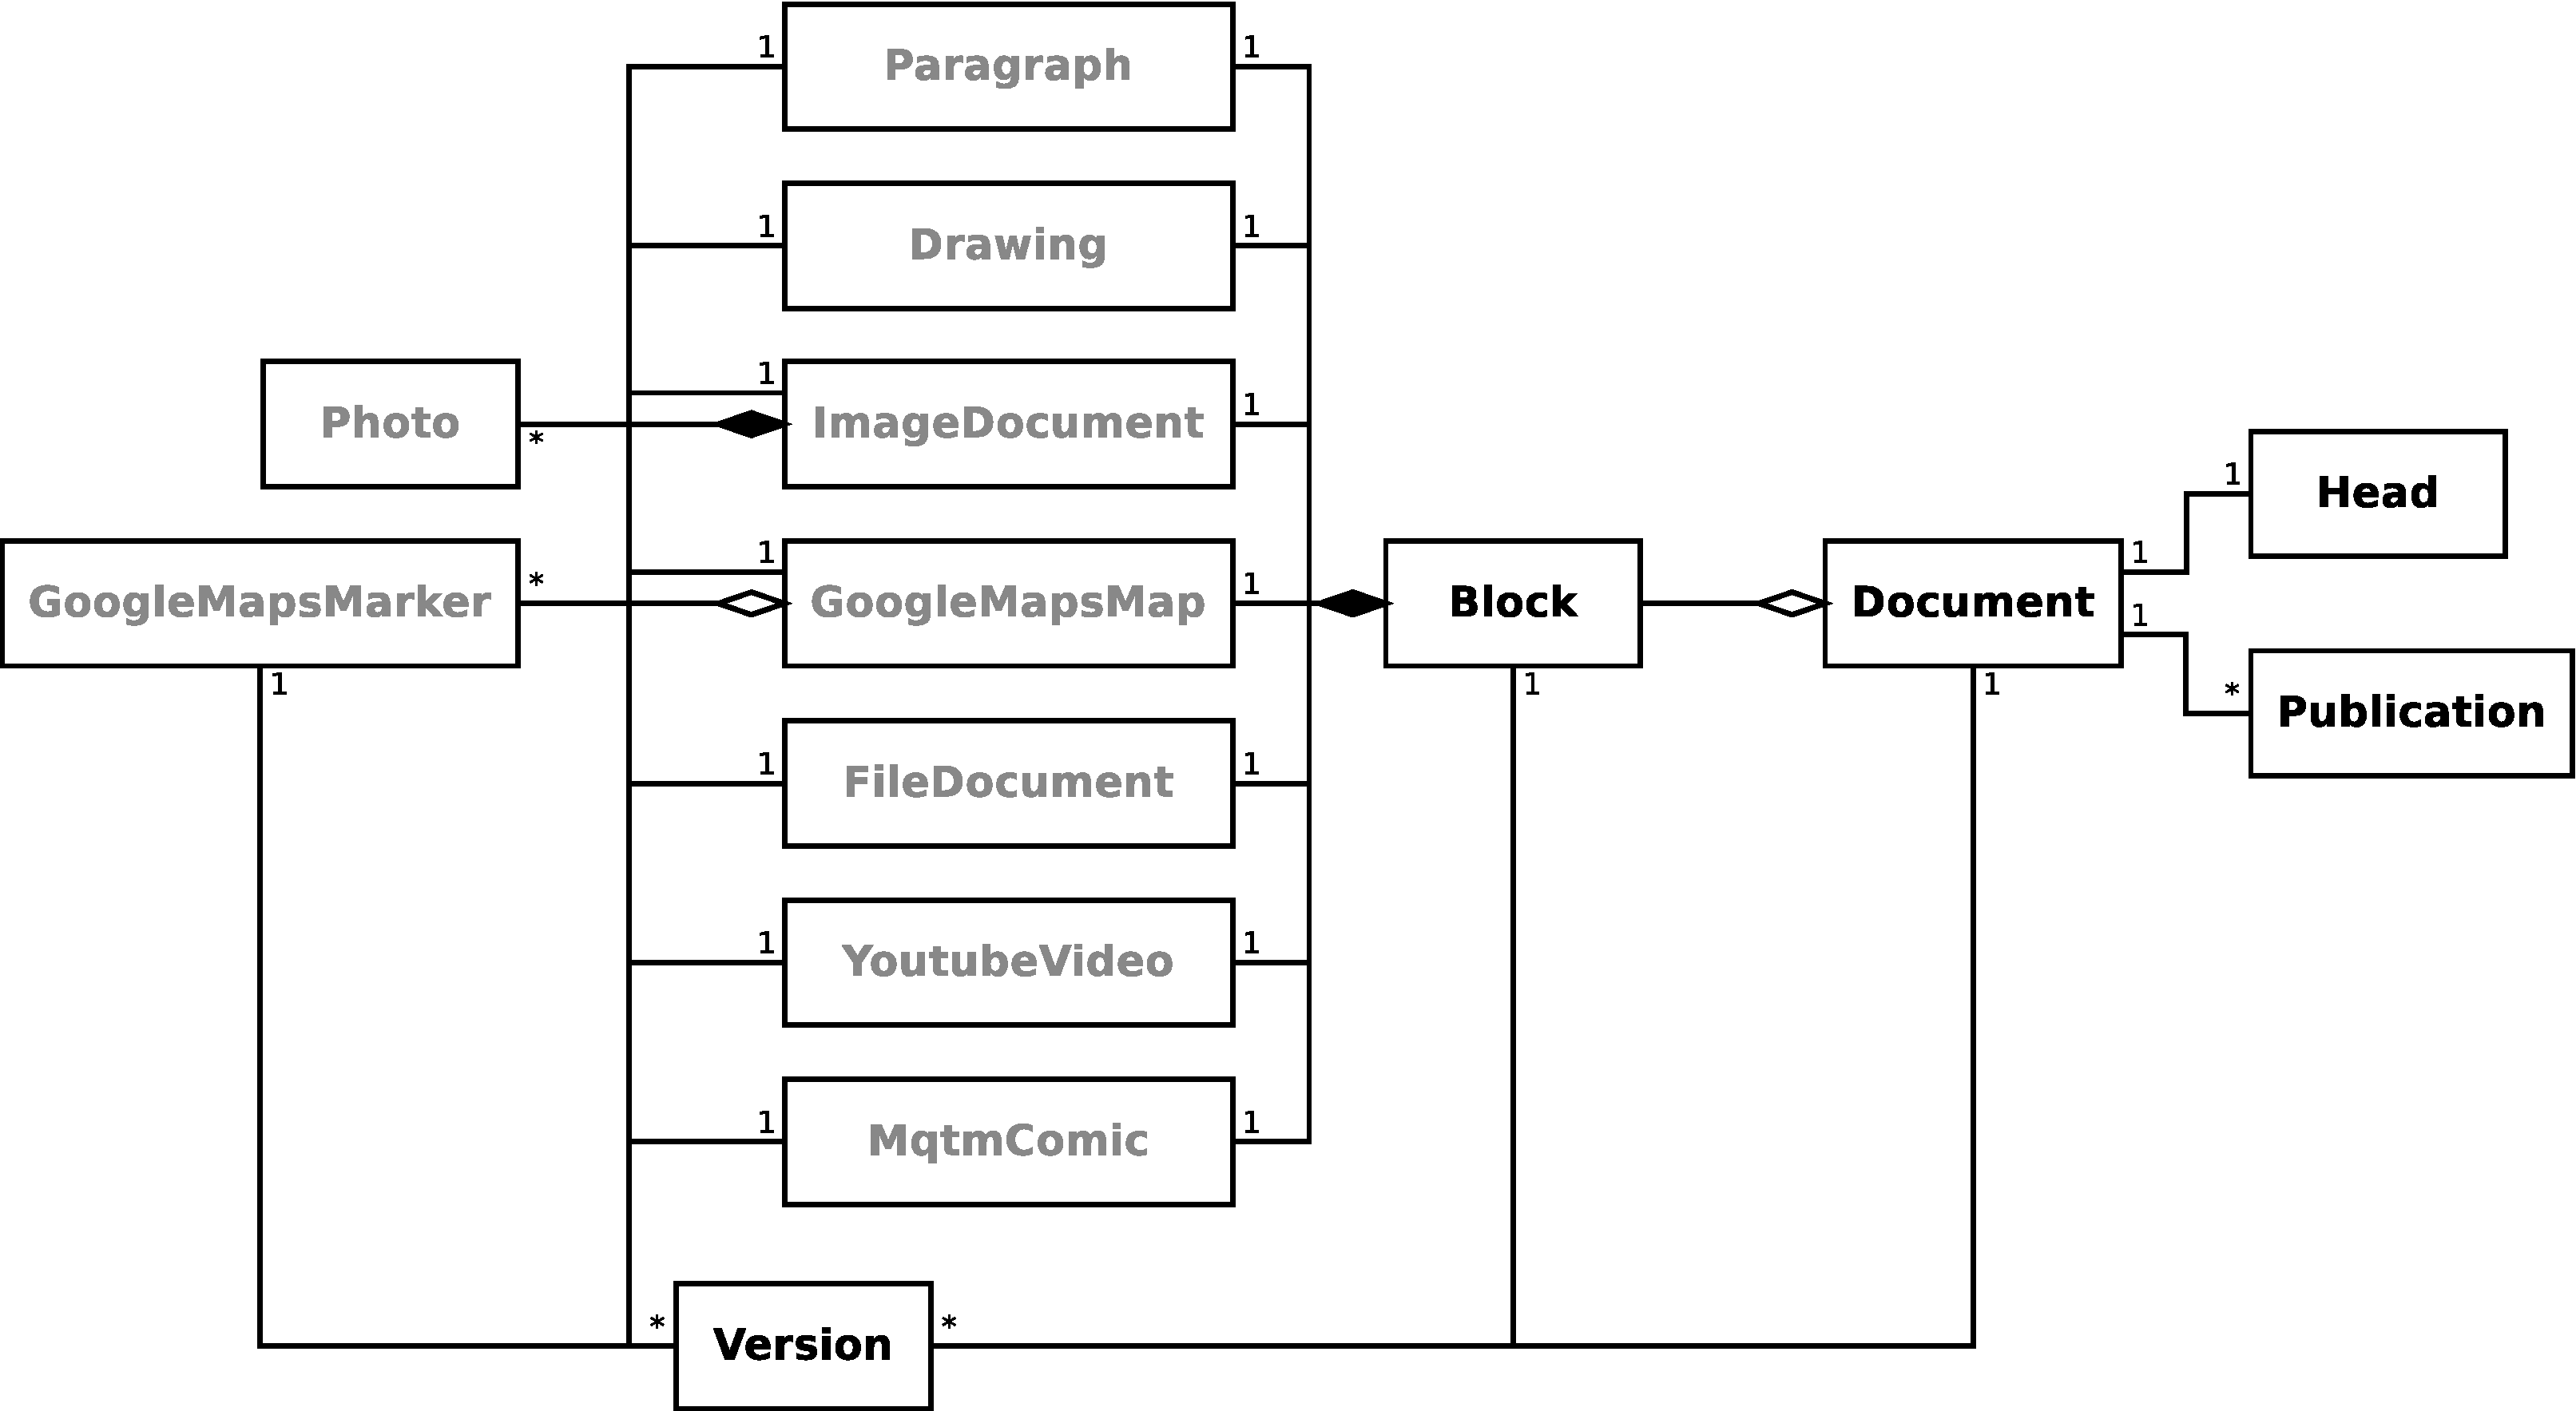
\includegraphics[width=165mm]{documents_current.pdf}
  \caption{Current Documents Model}
  \label{fig:documents_current}
\end{figure}

\subsection{Candidate Patterns}\label{sec:fa_documents_candidate_patterns}

\subsection{Chosen Patterns \& Rationale}\label{sec:fa_documents_chosen_patterns_rationale}

The pattern used is a composite design pattern as described in \cite{riehle_composite_patterns}, where various smaller design patterns work in tandem to create a more complex pattern:

\begin{itemize}
  \item \textsc{Memento} - used for versioning
  \item \textsc{Property} (simplified variant) - used for decoupling a \emph{Block content} from the database schema
  \item \textbf{INVESTIGATE: pattern 3} - the fact that a \emph{Publication} points to a specific \emph{Version} of a \emph{Document} may be a pattern --- it works as a \emph{tag} in a VCS (version control system) system such as git or SVN.
\end{itemize}

\begin{figure}[H]
  \centering
  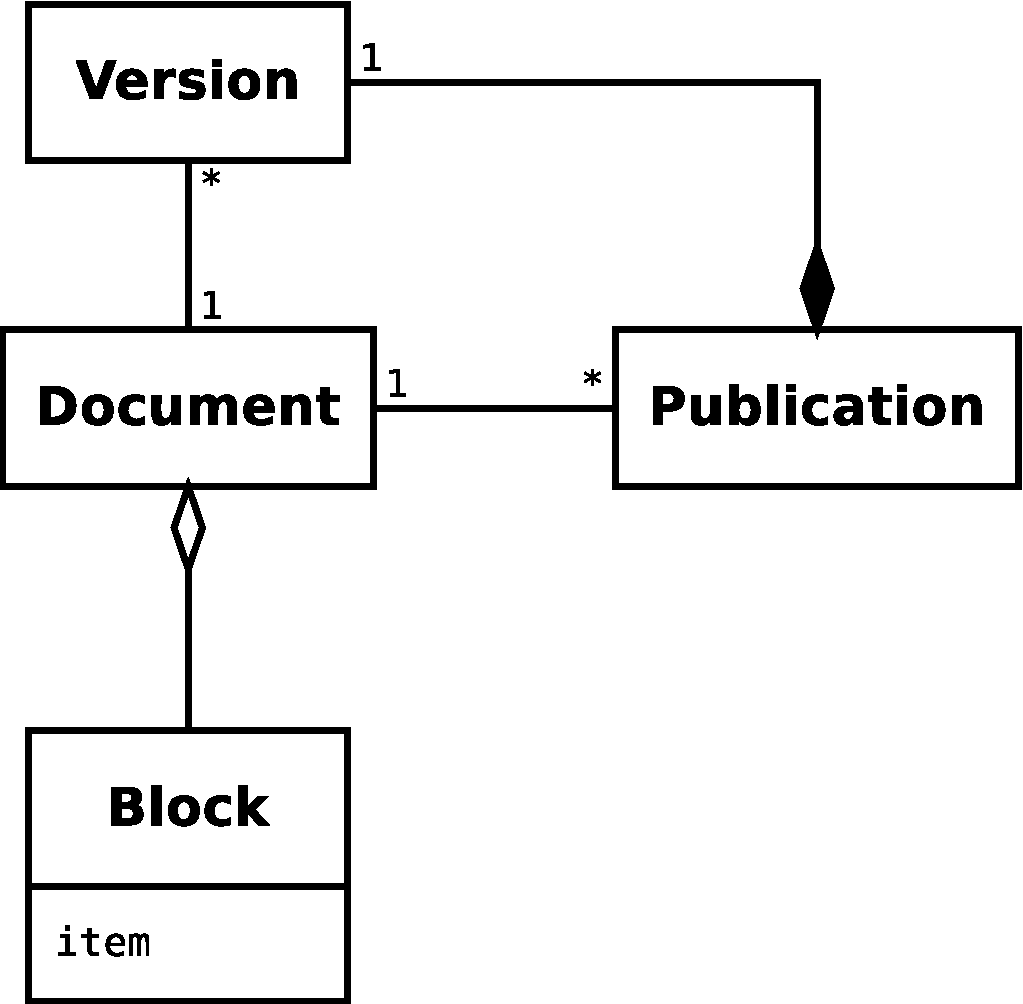
\includegraphics[width=75mm]{documents_conceptual.pdf}
  \caption{Conceptual Documents Model}
  \label{fig:documents_conceptual}
\end{figure}

The variant of the \textsc{Property} pattern implemented is simplified due to the highly dynamic nature of the Ruby language --- which means that, for this particular problem, it is able to build new types of objects or even create new class definitions in runtime, which allows discarding the \textsc{Property}--\textsc{PropertyType} pair (see \ref{sec:property_pattern}) in favour of a single entity, \emph{content}.

\subsection{Implementation}\label{sec:fa_documents_implementation}

The implementation of this composite pattern takes advantage of the highly dynamic nature of the Ruby language and the API provided by the \textsc{ActiveRecord} implementation of Rails.

\emph{Document}, \emph{Block}, \emph{Version} and \emph{Publication} are all AR objects, which means that, according to the AR pattern and the Rails framework conventions, each one of them is stored inside an SQL table, with a row for each one of the attributes. This structure provides the basic blueprint (as stated in \ref{sec:case-study_areas_document_editor}) for the documents to be produced by the editor --- it allows a title, an arbitrary number of orderable blocks, and a snapshot (version) of each modification. It also allows for publications, which essentially point to a specific version of a document.

There is nothing really remarkable about \emph{Blocks}, \emph{Documents} of even \emph{Publications} --- they are ordinary \textsc{ActiveRecord} objects, with associations to each other (as pictured in Fig.~\ref{fig:documents_conceptual}), and explaining how they work is outside of the scope of this study.

However, a \emph{Version} is a bit more complex than a simple AR object, in the sense that it contains a full representation of another AR object at a given point in time --- in this case, a \emph{Document}. This is achieved by serializing a \emph{Document} and all its associations (\emph{Blocks}) in the JSON format, which preserves all the necessary information needed to rebuild a specific \emph{Document} at whichever time that \emph{Version} refers to --- which means that a \emph{Version} effectively implements the \textsc{Memento} design pattern to keep a history of each \emph{Document}.

Finally, a \emph{Block} content possesses special properties that, together with AR, create a dynamic and variable foundation for the development of different types of content. As a \emph{Block} is simply a generic container for an arbitrary type of content, a \emph{Block} content can't be constrained to a single class or object type. The solution is to serialize the content inside the \emph{content} attribute of a \emph{Block}. This way, a \emph{Block} content is simply a string that represents a serialized object --- which can be de-serialized, accessed and modified at runtime. This means that, whichever a \emph{Block} content may be, the content itself is responsible for its representation and life cycle.

In order to further simplify and streamline the development, a \emph{DocumentItem} (super)class was created. This class serves as a staple for further specialization through inheritance, and handles cross-cutting concerns such as object initialization, default values and validations for each of these attribute's values. The need for a specific controller for each one of the different Block items has also been discarded in favour of a single controller, responsible for handling the user input regarding the modification of blocks and their content.

\subsection{Impact Analysis}\label{sec:fa_documents_impact_analysis}

The refactoring of the Document Editor infrastructure had two major points of impact: performance, and variability.


\subsubsection{Performance}

With the current foundation for the editor, the number of queries grows linearly with the number of blocks that constitute a document, as it is necessary to perform a query for each one the items related to each one of the blocks. The usage of eager loading is limited due to the polymorphic nature of the blocks and each respective content, which is unknown \emph{a priori}.

From an universe of 3990 documents currently residing in the system (representative of all the documents present in the system as of November 23rd, 2010), the graph present in Fig.~\ref{fig:queries_per_blocks_in_document} shows a linear growth in the number of queries necessary to render a Document: the number of queries necessary are directly proportional to the number of blocks in a document with a 1:1 ratio. Just like in \ref{sec:fa_social_network_impact_analysis}, this represents a serious performance issue: as the most used feature in the \emph{escolinhas.pt} platform, a sustainable growth is very difficult to achieve if the database load increases linearly with the number of existent Blocks in Documents.

\begin{figure}[H]
  \centering
  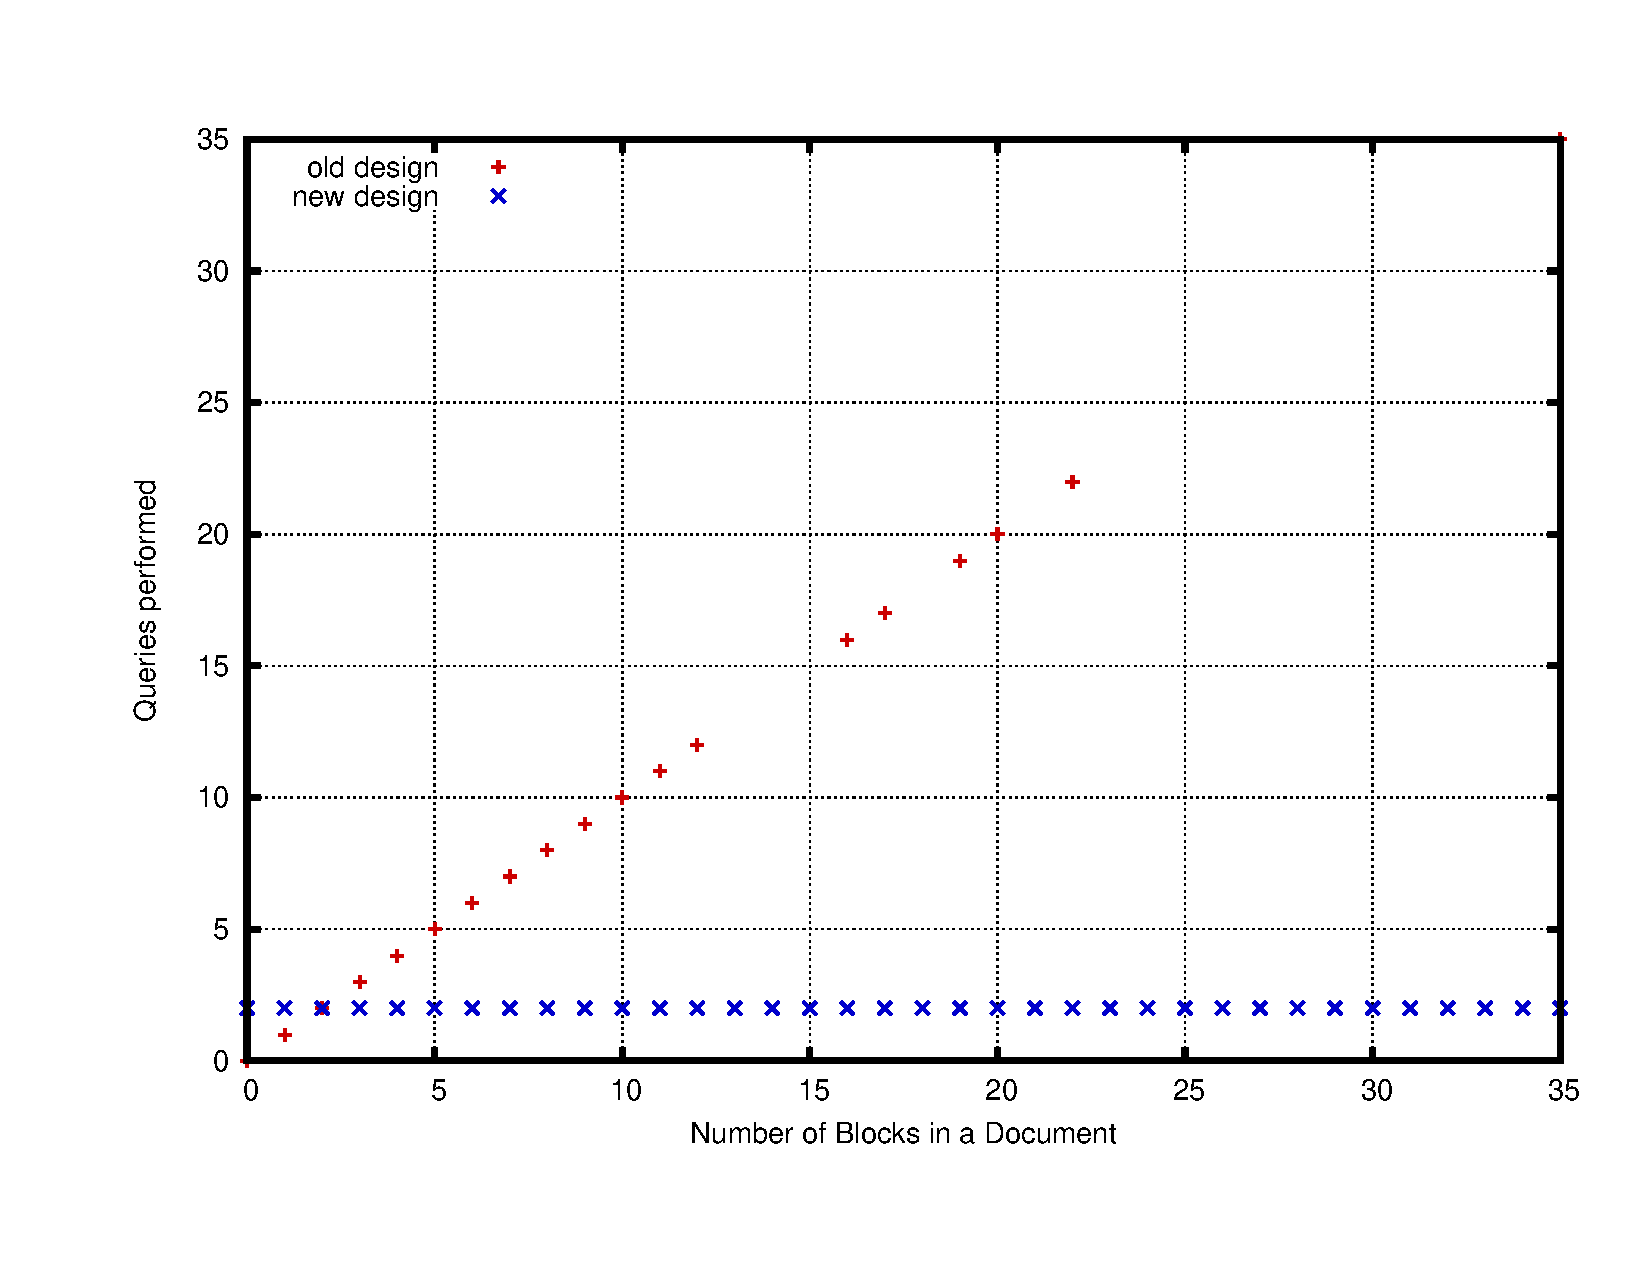
\includegraphics[width=145mm]{graphs/document_queries}
  \caption{Average number of queries performed per number of Blocks in a single Document}
  \label{fig:queries_per_blocks_in_document}
\end{figure}

The introduction of the model described in \ref{sec:fa_documents_chosen_patterns_rationale} makes the number of queries necessary to display a \emph{Document} to be constant (only 2 queries are performed), as only the Blocks and the Document itself are AR objects --- as the item that constitutes a Block is an integral part of a Block, no queries are necessary to fetch it.

\subsubsection{Variability}

Using the aforementioned infrastructure for the document editor, the work necessary to create new types of blocks has been greatly reduced. This allows for much shorter prototyping and testing iteration times --- no database schemas or migrations to worry about, allowing the developers to focus on the details of the model rather than implementation details --- which ultimately leads to a higher degree of variability.



